%\begin{document}
\chapter{RS码的编码与BM硬判决算法}
\thispagestyle{empty}
%==========================================================================
\section{RS码与水声通信}
由于前面已经介绍了卷积码,已经在水声通信中使用卷积码,而且理论和实际当中,同等复杂度运算量的卷积码要比RS码的误码率性能要好,为什么这里还要研究RS码,并且作为一种信道编码方式应用到水声通信中?

在第三章中介绍了卷积码编码中几种码的终结方式,而且本设计也根据通信要求和实际情况选择了终结和咬尾两种码终结方式的结合,这就是意味着,编码的总长度比实际数据码字长度要多一个约束长度$K$,对于数据量很大的情况下,约束长度$K$就显得微不足道了,可以忽略不计,并不会导致多少带宽的浪费和码率的下降,而对于命令等几个字节甚至是几个比特数据量的时候,这就显得不合适了,对于序贯译码方式,通常选择约束长度$K$都很大,对于本设计仿真我们采用的是$K=24$,就是3个字节,可能远比要传输的数据量大,因此造成了很大的带宽浪费。因此采用RS码。

\section{RS码概述}
RS\footnote{Reed-Solomon}码是由MIT林肯实验室的Irving~S.~Reed和Gustave~Solomon\cite{Reed_RS}于1960年提出的一种基于多项式的纠错编码,Gorenstein和Zierler于1961年证明了RS码与多进制BCH码的关系。Berlekmamp于1967年提出了直到至今还被广泛应用的硬判决译码算法,两年后,Massey指出了此算法和线性反馈移位寄存器的关系,因此,该硬判决译码算法被称为BM算法,一直沿用至今。

RS码具有很好的纠错特性,它是目前唯一实用的最小距离可分\footnote{MDS}码,能够有效地纠正随即符号错误,突发错误和删除错误。因此,在诞生初期,便被迅速应用。
%==========================================================================
\section{RS码的编码}
RS码是一种常见的线性分组码,同时它也是循环码。所谓循环码指的是任意码字循环移位后仍然在码字空间内的一类线性分组码\cite{Coding_Fundation}。

一个$(n,k)$循环码可以用$n-k$次的生成多项式$g(x)$定义,其码多项式$(n-1\mbox{次})c(x)$是$g(x)$的倍式:$c(x)=f(x)g(x),k-1$次多项式$f(x)$称为消息多项式,其$k$个系数就是$k$个消息码元。由第二章的知识可知,如果$g(x)$是$x^n-1$的因子,由$g(x)$生成的码一定是循环码。

通过定义生成多项式,RS码可以这样定义:在$GF(q)$上,$\alpha$为本原域元素,$g(x)$定义为:
\begin{eqnarray}
  g(x)=(x-\alpha)(x-\alpha^2)\cdots (x-\alpha^{2t})
  \label{equ:4.1}
\end{eqnarray}
其中$2t=n-k,n=q-1$

由第二章的知识可知,对$GF(q)$而言,所有的$q-1$个非零元素就是$x^{q-1}-1$的所有根。那么,显然$g(x)\mbox{是}x^n-1$的因子,因此,这样构造出来的码是循环码。

由\ref{equ:4.1}定义的RS码最小距离是$2t+1$,因此通过硬判决能纠正$t$个错误。RS码的一个特点就是能够通过调整\ref{equ:4.1}根的数量很方便地调整其纠错能力。

对于能够纠错$t$个错误的$RS(n,k,d)$码,具有如下特征:
\begin{enumerate}
  \item \textbf{码长:}$n=2^m-1$符号或$m(2^m-1)$比特;
  \item \textbf{信息码元数:}$k=n-2t$符号或$mk$比特;
  \item \textbf{监督码元数:}$n-k=2t$符号或$m(n-k)$比特;
  \item \textbf{最小距离:}$d=2t+1=n-k+1$符号或$m(n-k+1)$比特
\end{enumerate}
令信息码元多项式为:
\begin{eqnarray}
  m(x)=m_0+m_1x+m_2x^2+\cdots +m_{k-1}x^{k-1}
  \label{equ:4.2}
\end{eqnarray}
\subsection{基于乘法形式的RS编码器}
公式:$c(x)=m(x)g(x)$

结构图如下:
\begin{figure}[htbp]
  \begin{center}
    \includegraphics[width=0.8\textwidth]{images/RS1.pdf}
  \end{center}
  \caption{乘法编码器结构图}
  \label{fig:4.1}
\end{figure}
图\ref{fig:4.1}具体实现步骤如下:
\begin{enumerate}
  \item $2t$个寄存器全部清0;
  \item
    $m(x)$最高次系数$m_{k-1}$首先送入时,乘法器输出乘积的最高此项$x^{k+2t-1}$的系数$m_{k-1}g_{2t}$,同时$m_{k-1}$存入寄存器的第一级;
  \item
    $m(x)$的第二个系数$m_{k-2}$送入时,$m_{k-1}$由第一级进入第二级寄存器,同时与$g_{2t-1}$相乘,$m_{k-2}g_{2t}+m_{k-1}g_{2t-1}$就是得到的乘积$x^{k+2t-2}$的系数;
  \item 就这样重复进行,直到$k+2t$次移位后,乘法器输出乘积的常数项$m_0g_0$
\end{enumerate}
但是结构图\ref{fig:4.1}编码出来的RS码是非系统码,这并不是我们需要的,因此,下面将介绍系统码的编码器结构。
\subsection{基于除法形式的RS编码器}
设校验码多项式:
\begin{eqnarray}
  h(x)=h_kx^k+h_{k-1}x^{k-1}+\cdots +h_1x+h+0
  \label{equ:4.3}
\end{eqnarray}
系统码的多项式:
\begin{eqnarray} 
  C(x)=c_{n-1}x^{n-1}+c_{n-2}x^{n-2}+\cdots +c_{n-k}x^{n-k}+\cdots +c_1x+c_0
  \label{equ:4.4}
\end{eqnarray}
它的前$k$位系数:$c_{n-1},c_{n-2},\cdots
,c_{n-k}$是已知的信息位,而后$n-k$位系数:$c_{n-k-1},c_{n-k-2},\cdots
,c_1,c_0$是要求的校验位。码多项式必是生成多项式$g(x)$的倍式,所以
\begin{eqnarray}
  C(x)=m(x)g(x)
  \label{equ:4.5}
\end{eqnarray}
其中$\partial C(x)\le n-1,\partial g(x)=n-k,\partial m(x)\le k-1$
而
\begin{eqnarray}
  h(x)C(x)=m(x)g(x)h(x)=m(x)(x^n-1)=m(x)x^n-m(x)
  \label{equ:4.6}
\end{eqnarray}
由于中$\partial C(x)\le n-1,\partial g(x)=n-k,\partial m(x)\le
k-1$,所以$m(x)x^n$的最低位次数至少为$n$次,因而在$h(x)C(x)$的乘积中$x^{n-1},x^{n-2},\cdots
,x^k$的次数为0。

而根据式\ref{equ:4.6}最左边的乘积可知,$x^{n-1}$的系数:
\begin{eqnarray}
  c_{n-1-0}h_0+c_{n-1-1}h_1+\cdots +c_{n-1-k}h_k
  \label{equ:4.7}
\end{eqnarray}
同理,$x^{n-2}$的系数:
\begin{eqnarray}
  c_{n-2-0}h_0+c_{n-2-1}h_1+\cdots +c_{n-2-k}h_k
  \label{equ:4.8}
\end{eqnarray}
根据上边的分析,
\begin{eqnarray}
  \sum_{j=0}^kc_{n-i-j}h_j=0 \hspace{1.5cm}i=0,1,2,\cdots ,n-k
  \label{equ:4.9}
\end{eqnarray}
由于$h_k=1$,所以式\ref{equ:4.9}可以改写为:
\begin{eqnarray}
  c_{n-k-i}=-\sum_{j=0}^{k-1}c_{n-i-j}h_j \hspace{1.5cm}i=1,2,\cdots ,n-k
  \label{equ:4.10}
\end{eqnarray}
式\ref{equ:4.10}展开为:
\begin{eqnarray}
  \begin{array}{ll}
    c_{n-k-1}\hspace{8mm}=&-(c_{n-1}h_0+c_{n-2}h_1+\cdots +c_{n-k}h_{k-1})\\
    c_{n-k-2}\hspace{8mm}=&-(c_{n-2}h_0+c_{n-3}h_1+\cdots +c_{n-k-1}h_{k-1})\\
    \multicolumn{2}{c}{\vdots}\\
    c_{n-k-(n-k)}~\,=&c_0=-(c_kh_0+c_{k-1}h_1+\cdots +c_1h_{k-1})
  \end{array}
  \label{equ:4.11}
\end{eqnarray}
由上式看出码字$C$的第一个码元$c_{n-k-1}$可由$k$个信息元$c_{n-1},c_{n-2},\cdots
,c_{n-k}$与$h(x)$的系数相乘得到,而由$c_{n-2},c_{n-3},\cdots
,c_{n-k},c_{n-k-1}$可得到第二个校验元$c_{n-k-2}$,再由$c_{n-3},\cdots
,c_{n-k}$信息元和第一、第二校验元$c_{n-k-1},c_{n-k-2}$可得到第三校验元$c_{n-k-3}$。按这样的线性关系递推,一直可求得所有的$n-k$个校验元$c_{n-k-1},c_{n-k-2},\cdots
,c_1,c_0$。
\begin{figure}[htbp]
  \begin{center}
    \includegraphics[width=0.8\textwidth]{images/RS2.pdf}
  \end{center}
  \caption{除法编码器结构图}
  \label{fig:4.2}
\end{figure}
因此,基于校验多项式$h(x)$构造除法编码器结构图如\ref{fig:4.2}
由于此种结构图编码出来的码字是系统码,因此,在本设计中,采用的就是这种编码结构。
%==========================================================================
\section{RS码的译码}
就目前RS码的译码算法中,主要有硬判决算法和软判决译码算法,硬判决算法就是上面提到的Berlekamp-Massey(BM)算法,其纠错能力为$t\le
(d_{min}-1)/2,d_{min}=n-k+1$为最小汉明距离。

而软判决译码算法有如下几种:
\begin{enumerate}
  \item \textbf{由代数硬判决译码改进的准软判决译码算法}\footnote{GMD,Chase算法}:
    \quad
    由于删除信息可以看作最简单的软信息利用形式,Forney提出的GMD译码算法通过删除最不可靠的码字,多次运行BM算法来实现译码,可以看作是RS码的准软译码算法;Chase提出的Chase算法通过翻转最不可靠的码字后多次运行BM算法来实现译码。这两种算法的原理是很相似的,前者性能低,后者复杂度大。
  \item \textbf{代数软判决译码算法}\footnote{ASD:Algebraic Soft Decision 算法}
    \quad
    此类算法的代表就是Koetter和Vardy提出的KV算法\cite{KV_RS}。KV算法通过对不同的插值点分配不同的重数,将信道输出的软信息转换成代数约束条件,之后再执行GS\footnote{由Guruswami和Sudan提出的代数列表译码算法}算法\cite{GS_RS},实现了软判决译码。KV算法可以方便的调节参数,实现复杂度和性能的折中。
  \item \textbf{自适应的信度传播算法}\footnote{ABP:Adaptive Belief Propagation算法}
    \quad
    ABP算法由Jiang等人于2004年提出\cite{ABP_RS},它利用了在LDPC码译码中常用的BP算法。BP算法要求校验矩阵式稀疏的,而RS码进行二进制展开后的校验矩阵仍然是高密度的。Jiang通过在BP算法前对矩阵进行一定的处理,使其对应于置信度较低的矩阵式稀疏的,而后进行BP迭代,实现译码。
\end{enumerate}

介绍以上方式,只是说明RS码应用很广泛,译码方法很成熟,但是针对于水声通信来说,不需要这么复杂的软判决译码算法,而BM算法的简单,易实现特点很适合于水声通信。下面就Berlekmap-Massey详细讲解。
%==========================================================================
\section{Berlekmap-Massey硬判决算法}
%**************************************************************************
\subsection{Berlekamp-Massey迭代原理\cite{Jonathan_BCH}}
众所周知分组码最典型的硬判决译码方法就是伴随式(Syndrome)译码,译码分为三个步骤:
\begin{enumerate}
  \item 计算伴随式;
  \item 由伴随式求取错误图样
  \item 将错误图样与接收码字相加,得到译码输出
\end{enumerate}
在第二步中,又分为求取错误位置和求取错误值,而BM算法本质上是求取错误位置多项式,而利用钱搜索计算错误位置多项式的根,而Forney算法来计算错误值,这两个算法会在第四小节介绍。下面对BM算法的原理做些介绍\cite{ChenWenli_RS}。

把错误图样$\vec{e}$也看做一个多项式:
\begin{eqnarray}
  e(x)=e_0+e_1x+e_2x^2+\cdots +e_{n-1}x^{n-1}
  \label{equ:4.12}
\end{eqnarray}
假如实际发生的错误为$v,0\le v\le
t,t$为RS码纠错能力$(n-k=2t)$,那么,错误多项式就可以写成仅有$v$项的形式:
\begin{eqnarray}
  e(x)=e_{i_1}x^{i_1}+e_{i_2}x^{i_2}+\cdots +e_{i_v}x^{i_v}
  \label{equ:4.13}
\end{eqnarray}
其对应的错误图样的形式为:$\vec{e}=(0\cdots e_{i_1}\cdots 0 \cdots
e_{i_2}\cdots \cdots 0\cdots e_{i_v}\cdots 0)$,下标$i_l$在$0\sim
n-1$整数中取值,代表错误的位置,$l$在$1\sim v$取值。

知道,$\vec{V}=\vec{r}H^T=\vec{e}H^T$,代入RS码H矩阵的形式,则有:
\begin{eqnarray}
  \vec{S}=(0\cdots e_{i_1}\cdots 0 \cdots
  e_{i_2}\cdots 0\cdots e_{i_v})\left[\begin{array}{cccc}
    1&1&\cdots&1\\
    \alpha^1&\alpha^2&\cdots&\alpha^{2t}\\
    \left(\alpha^1\right)^2& \left(\alpha^2\right)^2&\cdots&
    \left(\alpha^{2t}\right)^2\\
    \vdots&\vdots&\vdots&\vdots\\
    \left(\alpha^1\right)^{n-1}& \left(\alpha^2\right)^{n-1}&\cdots&
    \left(\alpha^{2t}\right)^{n-1}
  \end{array}\right]
  \label{equ:4.14}
\end{eqnarray}
由矩阵乘法定义可知,$\vec{e}^T$和H的$2t$个列向量进行求内积运算,$\vec{e}^T$与第$j$个列向量求内积求出$\vec{S}$的第$j$个分量:
\begin{eqnarray}
  S_j=e_{i_1}\left(\alpha^j\right)^{i_1}+e_{i_2}\left(\alpha^j\right)^{i_2}+\cdots
  +e_{i_v}\left(\alpha^j\right)^{i_v}=e\left(\alpha^j\right),1\le j\le 2t
  \label{equ:4.15}
\end{eqnarray}
为了表达方便,假设$Y_l=e_{i_l},1\le l\le v$;设$X_l=\alpha^{i_l},1\le l\le
v$,事实上,$Y_l$就是错误图样中某个错误位置上的错误值,而$X_l$就代表着错误位置$i_l$,这样,上式\ref{equ:4.15}可以重写为:
\begin{eqnarray}
  S_j=Y_1X_1^j+Y_2X_2^j+\cdots +Y_VX_V^j,1\le j\le 2t
  \label{equ:4.16}
\end{eqnarray}
这可以看作一个方程组。设接收码字为$r(x)=c(x)+e(x)$,因为$\alpha^j,1\le j\le
2t$是$c(x)$的根:$c(\alpha^j)=0$,由由式\ref{equ:4.15},$r(\alpha^j)=e(\alpha^j)=S_j$,接收码字在接收端已知,可以求出$2t$个伴随式$S_j$,即完成伴随式译码的第一步。式\ref{equ:4.16}中未知的是$X_l,Y_l$的值,共$2v$个。$v\le
t$,可以通过解该方程组求得错误位置和错误值,但是这是个非线性方程组,求解过程非常复杂,因此采用先求错误位置,再求错误值。

定义次数为$v$错误位置多项式$\sigma(x)$:
\begin{eqnarray}
  \sigma(x)=1+\sigma_1x+\sigma_2x^2+\cdots
  +\sigma_vx^v=(1-X_1x)(1-X_2x)\cdots(1-X_vx)
  \label{equ:4.17}
\end{eqnarray}
这个定义表明,错误位置$X_l$的逆元$X_l^{-1}$是$\sigma(x)$的根。下面,目标就变成求$\sigma(x)$及其根。

可以证明\cite{Blahut_BM},$\sigma(x)$的系数与伴随式$S_j$之间存在如下关系:
\begin{eqnarray}
  \left[
  \begin{array}{cccc}
    S_1&S_2&\cdots &S_v\\
    S_2&S_3&\cdots &S_{v+1}\\
    \vdots &\vdots &\vdots &\vdots \\
    S_v&S_{v+1}&\cdots &S_{2v-1}
  \end{array}
  \right]
  \left[
  \begin{array}{c}
    \sigma_v \\
    \sigma_{v-1}\\
    \vdots \\
    \sigma_1
  \end{array}
  \right]=-
  \left[
  \begin{array}{c}
    S_{v+1}\\
    S_{v+2}\\
    \vdots \\
    S_{2v}
  \end{array}
  \right]
  \label{equ:4.18}
\end{eqnarray}
而Berlekamp提出了一种基于上式\ref{equ:4.18}迭代求$\sigma(x)$的方法,Massey\cite{Massey_BCH}发现了这种迭代算法和线性反馈移位寄存器的关系,因此,把这种实用的求解算法称为BM算法,下面研究BM迭代\cite{ER_BCH}求$\sigma(x)$的具体过程,式\ref{equ:4.18}的关系可以简写成:
\begin{eqnarray}
  S_j=-\sum_{i=1}^v\sigma(x)_iS_{j-i}=v+1,\cdots ,2v
  \label{equ:4.19}
\end{eqnarray}
第二章讲过,在$GF(2^m)$上的加法求逆和加法等价,因此,可以把负号可以省略。

式\ref{equ:4.19}可以等效成一个线性反馈移位寄存器(设$v=3$):
\begin{figure}[htbp]
  \begin{center}
    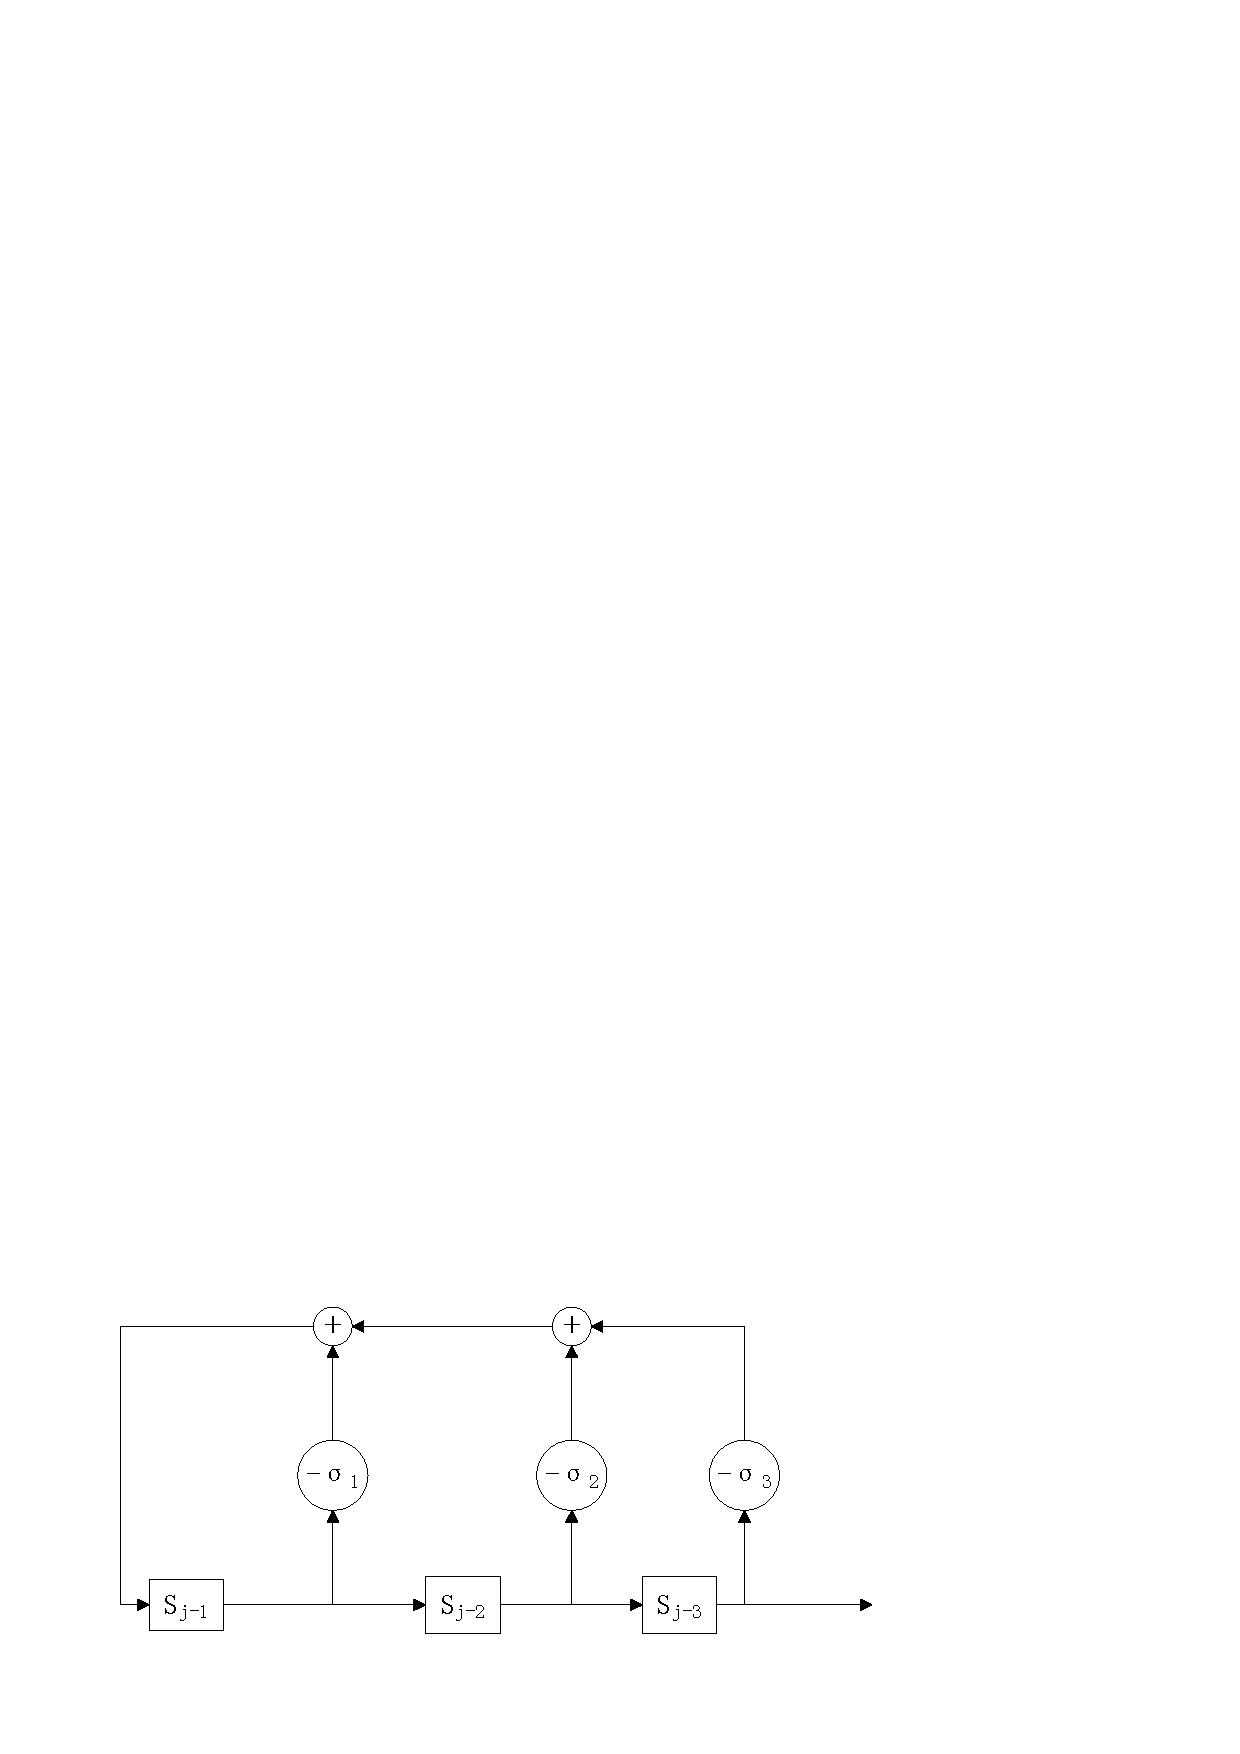
\includegraphics[width=0.6\textwidth]{images/BM.pdf}
  \end{center}
  \caption{BM迭代过程移位寄存器图}
  \label{fig:4.3}
\end{figure}

如果$\sigma_1,\cdots ,\sigma_v$已知,将寄存器中置入$S_1,\cdots
,S_v$的值,随着移位,在输出处就会产生$S_{v+1},\cdots
,S_{2v}$的值。现在的问题是,$S_1,\cdots
,S_{2t}$是知道的,$\sigma_1,\cdots
,\sigma_v$未知。可以采用迭代的方法构造出一个移位寄存器来符合上面的输入输出关系。注意到,$\sigma(x)$的系数就是寄存器的抽头权重。

可以用数学归纳法完成对迭代过程的推导。假设,第$r-1$次迭代,寄存器长度$L_{r-1}$,此时的寄存器抽头权重为$\sigma^{r-1}(x)$,它能够保证产生准确的$S_1,\cdots
,S_{r-1}$。下面的问题是怎么产生$\sigma^r(x)$能够使它能产生$S_1,\cdots
,S_r$。当抽头权重为$\sigma^{r-1}(x)$,前$r-1$次移位,产生了$S_1,\cdots
,S_{r-1}$,第$r$次移位,输出端的值记作$S_r'$:
\begin{eqnarray}
S_r'=-\sum_{j=1}^{D(r-1)}\sigma_j^{r-1}S_{r-j}  
  \label{equ:4.20}
\end{eqnarray}
其中$D(r-1)=\deg\sigma^{r-1}(x)$。它可能不等于$S_r$,定义它们的差值:
\begin{eqnarray}
  \Delta_r=S_r-S_r'=S_r+\sum_{j=1}^{D(r-1)}\sigma_j^{(r-1)}S_{r-j}=\sum_{j=0}^{D(r-1)}\sigma_j^{(r-1)}S_{r-j}
  \label{equ:4.21}
\end{eqnarray}
如果$\Delta_r=0$,说明$\sigma^{r-1}(x)$也能够正确地产生$S_r$,那么$\sigma^r(x)=\sigma^{r-1}(x)$,否则,要对抽头系数做个修正:
\begin{eqnarray}
  \sigma^{(r)}=\sigma^{(r-1)}(x)+Ax^l\sigma^{(m-1)}(x)
  \label{equ:4.22}
\end{eqnarray}
这里的$\sigma^{(m-1)}(x)$是前面$r-1$次迭代里出现过的一个多项式,$l$是一个整数,$A$是一个有限域元素,它们的选择我们下面再分析,选择它们的依据就在于它们的值能够让系数修正以后的$\Delta_r'=0$。

对这个新的多项式$\sigma^r(x)$,它的输出和$S_r$的差值为:
\begin{eqnarray}
  \Delta_r'=\Delta_r+A\sum_{j=0}^{D(m-1)}S_{r-j-l}
  \label{equ:4.23}
\end{eqnarray}
可以选择前面迭代过程中出现过的一个多项式$\sigma^{m-1}(x)$,满足$\Delta_m\neq
0$,令$l=r-m$,则上式\ref{equ:4.23}第二项变成了$A\Delta_m$,再选择$A=-\Delta_r/\Delta_m$,则有:
\begin{eqnarray}
  \Delta_r'=\Delta_r-\frac{\Delta_r}{\Delta_m}\Delta_m=0
  \label{equ:4.24}
\end{eqnarray}
这样就满足了$\Delta_r'=0$的条件,即:$\sigma^r(x)$能够产生$S_r$。可以证明,$S_1,\cdots
,S_r$同能也能够由$\sigma^r(x)$产生,事实上,式\ref{equ:4.22}可以看作把$\sigma^{m-1}(x)$连接在$\sigma^{r-1}(x)$上的辅助寄存器,当$\sigma^r(x)$进行前$r-1$移位时,它始终产生0,只有在第$r$次移位时,产生一个非零值$\Delta_m$,经过系统$A$修正后,正好用来补偿$\sigma^{r-1}(x)$的输出,使其输出$S_r$,这就是通过修正的方法产生$\sigma^r(x)$的基本思想。

如果只按照上面的说明,这样的$\sigma^{m-1}(x)$不是唯一的,这是不允许的。在BM算法中有一个约束条件\cite{Cheng_BCH},就是$\sigma^r(x)$的次数要尽可能低,因为$\sigma(x)$的次数就是错误的个数,在译码时总认为错误少的概率比错误多的概率高。事实上,在陪集首译码中作为陪集首的错误图样也要求重量尽可能轻,也是一样的道理。这些都是为了保证我们的译码是最小距离译码,即选择于接收码字汉明距离最小的码字作为译码输出。为了满足这个条件,在选择$m$的时候,需要选择的是出现在$\sigma^{r-1}(x)$前面,刚刚改变长度的那个$\sigma^{m-1}(x)$,即$L_{r-1}=L_M>L_{m-1}$。这样可以保证产生的$\sigma^r(x)$始终次数最低。经过这样的迭代,迭代$2t$次,就可以得到最终的错误位置多项式$\sigma^r(x)$。

%**************************************************************************
\subsection{BM算法的主要步骤及实现\cite{Nadia_BCH}}
下面,给出BM迭代的流程图\ref{fig:4.4}。流程图中的$B(x)$相当于前面说的$\sigma^{m-1}(x)$,两者只相差一个系数,而这个系数实际上是原来系数A里面分配了义部分。计算$T(x)$的多项式实际上就是式\ref{equ:4.20}。
\begin{figure}[htbp]
  \begin{center}
    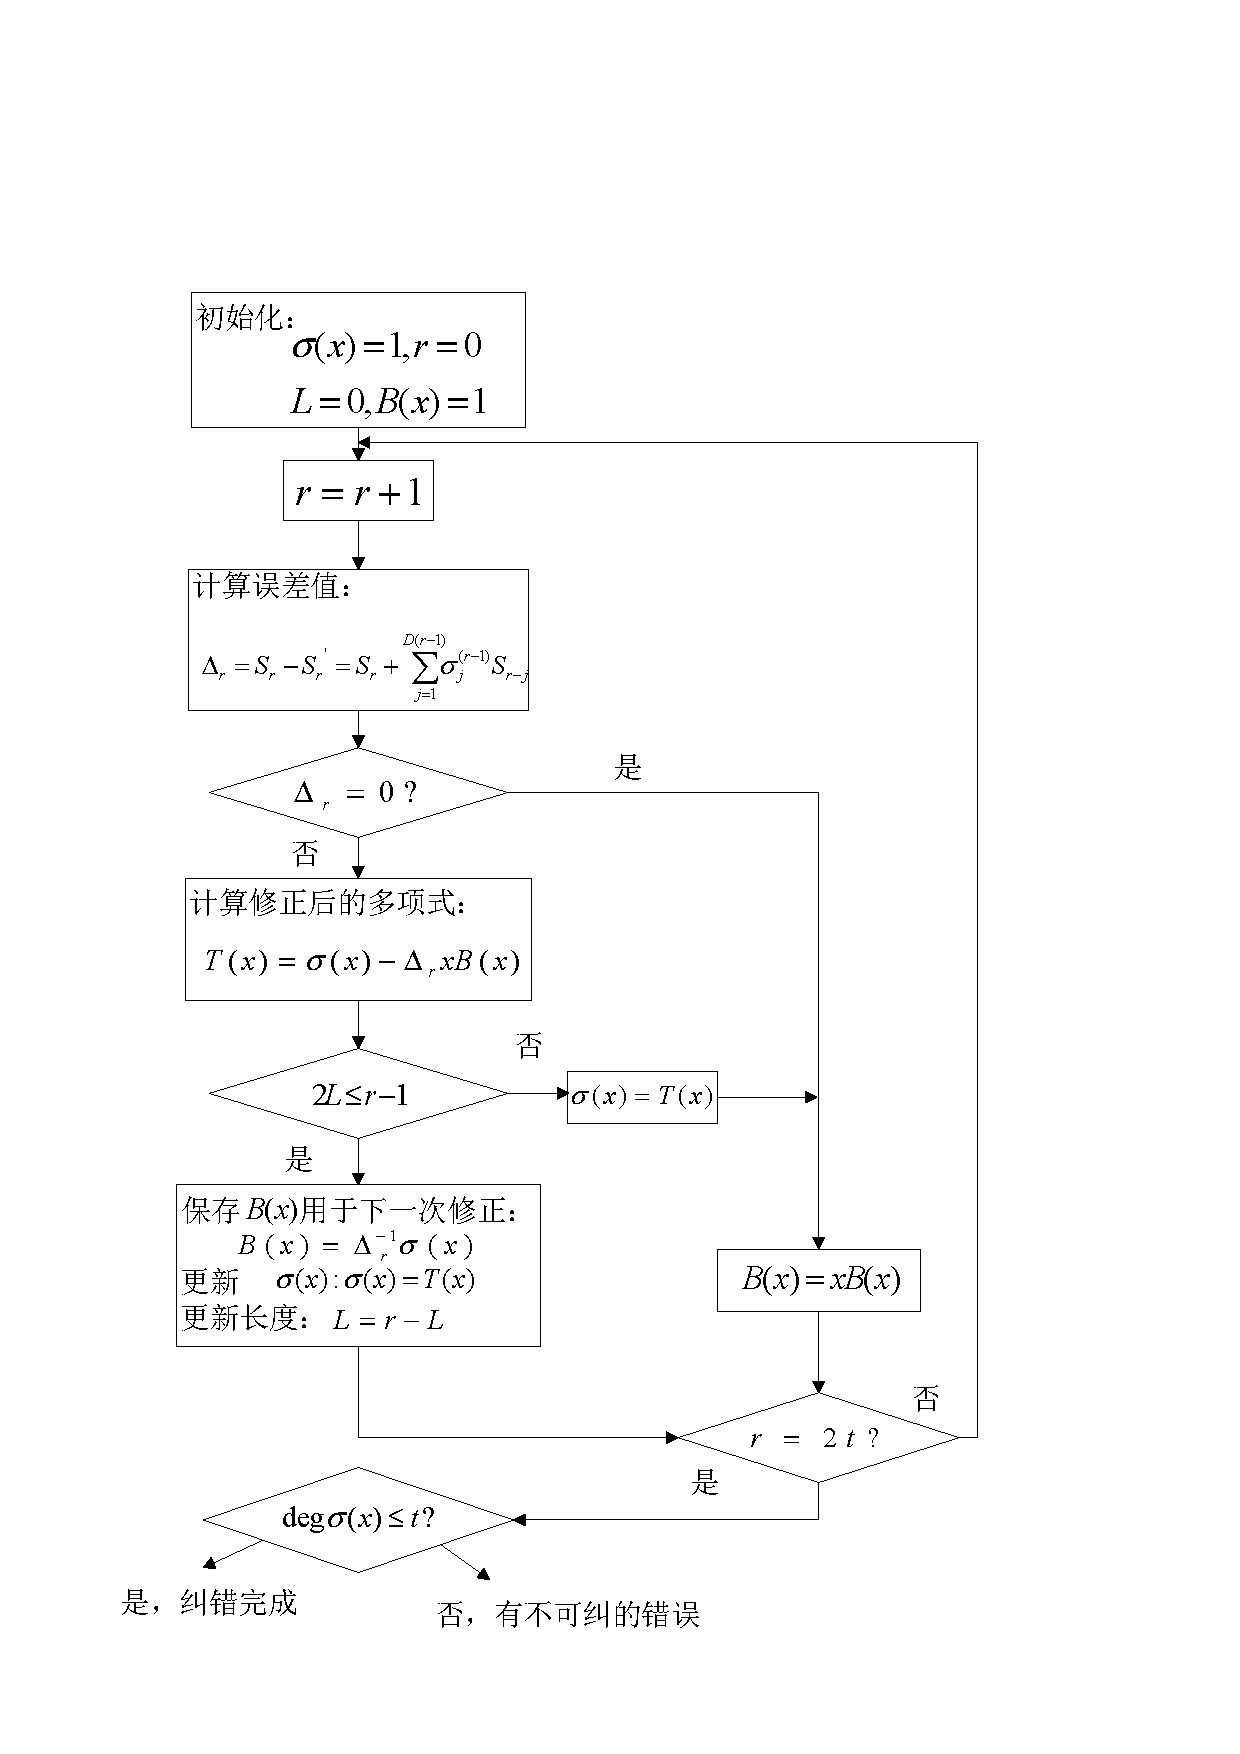
\includegraphics[width=0.6\textwidth]{images/BM1.pdf}
  \end{center}
  \caption{BM迭代流程图}
  \label{fig:4.4}
\end{figure}
具体步骤分析如下:
\begin{enumerate}
  \item 初始化:$\sigma(x),r=0,L=0,B(x)=1$,然后开始迭代$r=r+1$;
  \item
    按$\Delta_r=S_r+\sum_{j=1}^{D(r-1)}\sigma_j^{(r-1)}S_{r-j}$计算$\Delta_r$,若$\Delta_r=0$,则有$B(x)=xB(x)$,并计算$\Delta_{r+1}$,再进行下一次迭代;
  \item 若$\Delta_r\neq
    0$,计算修正后的多项式$T(x)=\sigma(x)-\Delta_rxB(x)$,若$2L\le
    r-1$不成立,则$\sigma(x)=T(x),B(x)=xB(x)$,如果成立,继续;
  \item
    保存$B(x)$用于下一次修正$B(x)=\Delta_r^{-1}\sigma(x),\sigma(x)=T(x),L=r-L$,判断$r=2t$,如果否,再进行下一次迭代;如果是,继续;
  \item 如果$\sigma(x)$的最高次数小于等于$t$那么纠错完成,否则,不可纠错。
\end{enumerate}
%==========================================================================
\subsection{钱搜索与Forney算法}
求得$\sigma(x)$,下一步的问题就是求得多项式的根。工程上使用钱搜索方法来确定错误位置,钱搜索的原理在于有限域的元素是有限域的。可以逐个代入进行验证。
这部分比较容易理解,在此做简要说明
\begin{eqnarray}
  \begin{array}{ll}
  \sigma(x)&=(1-X_1x)(1-X_2x)\cdots (1-X_vx)\\
  &=\prod\limits_{l=1}^v(1-X_lx)=\sigma_vx^x+\sigma_{v-1}x^{v-1}+\cdots
  +\sigma_1x+\sigma_0
\end{array}
  \label{equ:4.25}
\end{eqnarray}
首先验证位置$x^0$是否有错误,即把$x=\frac{1}{\alpha^0}=\alpha^n(\alpha^n=1)$代入$\sigma(x)$若结果等于0,说明第一个码元有错误,否则第一个码元是正确的。

把$x=\frac{1}{\alpha^1}=\alpha^{n-1}$代入$\sigma(x)$,验证位置$x^1$是否有错误。同理把$\alpha^{n-2},\alpha^{n-3},\cdots
,\alpha$代入$\sigma(x)$分别验证位置$x^2,\cdots ,x^{n-1}$是否错误。

下面还需要求取错误值$Y_l$,这里利用的是Forney算法。定义错误值多项式:
\begin{eqnarray}
  \Omega(x)=S(x)\sigma(x)\mod x^{2t}
  \label{equ:4.26}
\end{eqnarray}
这个式子又可以称作关键方程,其中$S(x)=1+S_1x+S_2x^2+\cdots
+S_{2t}x^{2t}$,通过上面的步骤,求得了$S(x)$和$\sigma(x)$,因此$\Omega(x)$可以很快求出,而$\Omega(x)$还可以写为\cite{Blahut_BM}:
\begin{eqnarray}
  \Omega(x)=x\sum_{i=1}^vY_iX_i\prod\limits_{l\neq i}(1-X_lx)
  \label{equ:4.27}
\end{eqnarray}
将$\sigma(x)$的某个根$X_l^{-1}$代入,就可以求出对应位置的错误值:
\begin{eqnarray}
  Y_l=\frac{\Omega(X_l^{-1})}{\prod\limits_{j\neq l}(1-X_jX_l^{-1})}
  \label{equ:4.28}
\end{eqnarray}
这样,错误图样就被确定,将接收码字和错误图样相加,就得到了译码码字。
%**************************************************************************
\subsection{BM算法性能仿真}
通过matlab仿真信道特性以及调制方式,而C语言实现编译码方式,最后得到的数据在matlab里编程画出误码率曲线图。

图\ref{fig:4.5}是$RS(15,9,7)$码在PSK调制方式下的误码率仿真图。
\begin{figure}[htb]
  \begin{center}
    \includegraphics[width=\textwidth]{images/RS_BPSK.pdf}
  \end{center}
  \caption{$RS(15,9,7)$在PSK调制下误码率曲线图}
  \label{fig:4.5}
\end{figure}

从图\ref{fig:4.5}可以看出:RS码BM译码算法比未编码的信道误码率要好的多。

$E_b/N_0$低于4.75的时候,未编码比编码效果好,这是一种误解,因为RS码是多进制码,而本设计采用的是四进制,因此,在相同信号幅值和噪声的情况下,未编码码的$E_b/N_0$是RS码的四倍,即未编码在$E_b/N_0=1$的误码率应该还RS码$E_b/N_0=4$的误码率相比,从图中可以看出,还是RS码误码率低。


 
%**************************************************************************
\section{本章小结}
本章从RS码概述,编码器,译码器设计等方面介绍了RS码,其中编码器讨论了乘法形式的编码器和除法形式的编码器,而我们采用的是基于$h(x)$除法形式的编码器,因为,这种方式编出来的码字是系统码,然后从理论和具体实现步骤上介绍了BM算法,当然,为了译码完整,还简单介绍了用于求错误位置的钱搜索和求错误值的Forney算法,最后仿真验证性能。
%==========================================================================
%%========================================================================
% empty page for two-page print
\ifthenelse{\equal{\ioaside}{T}}{%
  \newpage\mbox{}%
  \thispagestyle{empty}}{}
%%========================================================================
%\end{document}
